% Example LaTeX document for GP111 - note % sign indicates a comment
\documentclass[12pt]{article}
% Default margins are too wide all the way around. I reset them here
\usepackage{amsmath}
%\usepackage{mathtools}
\usepackage{graphicx}
\usepackage[danish]{babel}
\usepackage{listings}
\usepackage{color}
\usepackage[utf8]{inputenc}
\usepackage{hyperref}
\numberwithin{equation}{section}

%\pagestyle{headings}

\definecolor{codegreen}{rgb}{0,0.6,0}
\definecolor{codegray}{rgb}{0.5,0.5,0.5}
\definecolor{codepurple}{rgb}{0.58,0,0.82}
\definecolor{backcolour}{rgb}{0.95,0.95,0.92}
 
\lstdefinestyle{mystyle}{
    backgroundcolor=\color{backcolour},   
    commentstyle=\color{codegreen},
    keywordstyle=\color{magenta},
    numberstyle=\tiny\color{codegray},
    stringstyle=\color{codepurple},
    basicstyle=\footnotesize,
    breakatwhitespace=false,         
    breaklines=true,                 
    captionpos=t,                    
    keepspaces=true,                 
    numbers=left,                    
    numbersep=5pt,                  
    showspaces=false,                
    showstringspaces=false,
    showtabs=false,                  
    tabsize=2
}
 
\lstset{style=mystyle}
\renewcommand\lstlistingname{Fil}
\renewcommand{\abstractname}{Hej}



\begin{document}
\title{Forberedelse til SRP-vejledning}
\author{Søren Fritzbøger 3F\\
HTX Hillerød}
%\renewcommand{\today}{}
\maketitle

%\begin{abstract}
%This article demonstrates a basic set of LaTeX formatting commands.
%Compare the typeset output side-by-side with the input document.smøøre
%\end{abstract}
%\tableofcontents
\section{Spørgsmål}
\emph{Jeg har fået følgende spørgsmål stillet af Christian, som er min vejleder i IT}

\begin{itemize}
\item Lav en kort (30-40 linjer) beskrivelse af dit emne.
\item Besvar de fem spørgsmål i pentagonen:
\begin{enumerate}
\item Hvad spørger du om? (Hvad er din problemformulering)?
\item Hvorfor spørger du? (Hvad er de faglige problemstillinger? Hvad er interessant? Hvad undrer du dig over?)
\item Hvad spørger du til? (Hvilket materiale skal du arbejde med? Hvad skal du
analysere?)
\item Hvad spørger du med? (Hvilke metoder vil du anvende?)
\item Hvordan vil du gå frem?(Hvordan vil du strukturere og disponere din opgave?)
\end{enumerate}
\item Skriv en foreløbig kommenteret kildeliste
\end{itemize}

Disse spørgsmål vil jeg besvare på næste side.

\newpage
\section{Besvarelse}
\subsection{Beskrivelse af emne}
Jeg har valgt at skrive om \emph{Numerisk Integration} i mit Studieretningsprojekt. Numerisk integration er en metode hvor man tilnærmelsesvist kan bestemme arealet under en funktion\emph{(graf)}. Normalt bruger man bestemte integraler til dette, men når funktionen er så avanceret, som f.eks. $f(x)=e^{-x^2}$, er det ikke muligt at bruge bestemt integration til at finde arealet.
Numerisk integration opdeler funktionen i mindre stykker, og udregner herefter arealet af dem og finder summen. Der findes flere forskellige metoder til at udregne arealet, og den mest simple af dem er midtpunktsreglen. Midspunktsreglen opdeler funktionen i en masse små rektangler, som er nemme at udregne arealet på. Metoden er som nævnt meget simpel, hvilket desværre også afpsejler sig i præcisionen, som man kan se på Figur 1.
\begin{figure}[hbtp]
\caption{Midpunktsreglen}
\centering
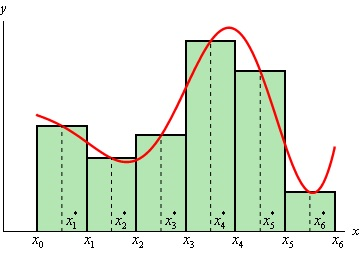
\includegraphics[scale=0.8]{midtpunktsreglen.jpg}
\end{figure}

Der findes også to andre metoder, henholdsvis trapez-metoden og simpsons-metode.\\
\textbf{Trapezmetoden} er en del mere avanceret. I stedet for at dele funktionen op i rektangler deler den funktionen op i trapezer. Som man måske kan se på Figur 2, er denne metode mere præcis end midtpunktsreglen.
\begin{figure}[hbtp]
\caption{Trapezmetoden}
\centering
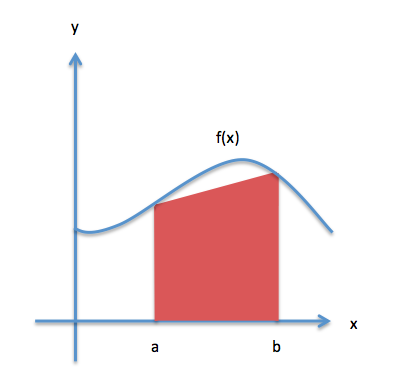
\includegraphics[scale=1]{trapezmetoden.png}
\end{figure}

Den sidste metode er simpsonsreglen, som virker ved at dele funktionen op i mindre og mere simple parabler, som man så finder arealet under.

\subsection{Hvad spørger jeg om}
\label{sec:hvad}
Jeg har udarbejdet en række spørgsmål som kan bruges til at udarbejde en problemformulering:
\begin{itemize}
\item funktioner og integraler
\begin{itemize}
\item Hvordan beskrives en funktion matematisk?
\item Hvad er integration af en funktion, og hvad er forskellen på bestemt og ubestemte integraler?
\item Hvordan kan integraler bruges til at udregne arealet af en funktion?
\end{itemize}

\item Forskellige metoder
\begin{itemize}
\item Hvordan ser de forskellige regler ud
\item Hvordan er deres præcision
\end{itemize}

\end{itemize}

\subsection{Hvorfor spørger jeg}
\label{sec:hvorfor}
Jeg skal jo relatere min matematik til IT, og det er heldigsvis nærliggende ved Numerisk Integration. De fleste matematikprogrammer som CAS, Mathcad eller lign. bruger Numerisk Integration til at udregne arealet under funktioner.
\subsection{Hvad spørger jeg til}
Jeg skal arbejde med en masse matematiske formler og udledningen af beviser. Samtidig skal jeg programmere noget der kan udregne arealet under grafer. Enten et program til computeren, en smartphone-app eller en hjemmeside. Så derfor skal jeg også arbejde med et programmeringssprog. Jeg skal selvfølgelig analysere metoderne og deres præcision.
\subsection{Hvad spørger jeg med}
Jeg er i tvivl om spørgsmålet og hvad der egentlig menes med det, men har prøvet at besvare det på den måde jeg tolker det som.
\\
Jeg vil undersøge forskellige metoder til at løse numerisk integration, herunder midtpunktsreglen, trapezreglen og måske simpsonsreglen, og undersøge deres præcision. For at inddrage IT vil jeg programmere et program, der vha. en af metoderne kan udregne arealet af en funktion.

\subsection{Hvordan vil jeg gå frem}
Opbygningen af matematikdelen passer med afsnit \emph{2.2 Hvad spørger jeg om}. Udover matematikdelen skal der være en IT-del, hvor jeg vil beskrive de metoder jeg bruger i programmet og forklare kildekoden.


\clearpage
\addcontentsline{toc}{section}{Litteratur}
\begin{thebibliography}{9}

\bibitem{JohnsonUtah}
  	Christopher R. Johnson,
  	\emph{Denne kilde er et dokument med beviser, beskrivelse og andet af numerisk integration.}.\\
  	Hamlet Project, 
  	Department of Computer Science,
	University of Utah,
	\url{http://www.cs.utah.edu/~zachary/computing/lessons/uces-13/uces-13/contents-node1.html}
	
\bibitem{html5canvas}
	@mattmight,
	\emph{En ``tutorial'' der viser hvordan man tegner en graf vha. html5 og canvas}.\\
	http://matt.might.net/articles/rendering-mathematical-functions-in-javascript-with-canvas-html/

\bibitem{au}
	Aalborg Universitet,
	\emph{Et foredag fra Aalborg Universitet omhandlende Numerisk Integration}.\\
	http://staff.iha.dk/jse/bioproces/Forelaesningsnoter/BI1MAT1/\\Numeriske\%20metoder\%201.pdf

\end{thebibliography}

\end{document}